% ---------------------------------------------------------------------------
% CURRENT RESULTS — drop-in section (requires: graphicx, booktabs).
% Place closed_loop_traces.png and openloop_drift.png in the graphics path.
% ---------------------------------------------------------------------------
\section{Current Results}

\subsection{Datasets}
All experiments use 1{,}000 simulated demonstrations (Newton physics, servo-plant arm,
Gaussian-splat rendering + Difix) of RJ45 cable insertion, evaluated closed-loop in the
same simulator (450-step budget; success = 11\,mm insertion depth inside a
$\sim$3\,mm-tolerance bore). Three variants of the training set exist:
\emph{original} (165{,}834 frames; the scripted expert decelerates to
$\sim$0.02\,mm/frame at its $-19$\,mm pre-dock standoff, leaving near-zero action
labels there), \emph{depaused} (arc-length resampled at a 0.2\,mm motion floor;
23.1\% of frames cut, actions recomputed across cuts), and \emph{dp01}
(gentler 0.1\,mm floor; 10.8\% cut, preserving the slow fine-alignment regime;
untested as of this writing).

\subsection{Open-loop probes}
Per-step imitation on training frames is near-perfect for every model
(Table~\ref{tab:probe}); open-loop metrics do not predict closed-loop behavior.

\begin{table}[h]\centering\small
\begin{tabular}{lllll}
\toprule
model & data & dpos err (mm) & direction cos & min $\lVert$pred$\rVert$ (mm) \\
\midrule
$\pi_{0.5}$ step 19999 & original & 0.088 & 0.853 & $\sim$0 at standoff \\
$\pi_{0.5}$ step 21000 & depaused & 0.096 & 0.918 & 0.212 \\
ACT c10 (15k)          & original & 0.105 & 0.800 & 0.052 \\
ACT c100 (100k)        & original & \textbf{0.037} & \textbf{0.974} & 0.031 \\
ACT c10 (15k)          & depaused & 0.146 & 0.810 & 0.148 \\
\bottomrule
\end{tabular}
\caption{Open-loop probe: first predicted action vs.\ ground truth on stride-sampled
frames of one training episode.}
\label{tab:probe}
\end{table}

Accumulating each model's prediction error \emph{along the expert path}
(teacher-forced; Fig.~\ref{fig:drift}) separates the failure sources: only the
paused $\pi_{0.5}$ carries a large systematic bias (4.5\,mm --- the stall);
every other model accumulates $<$1\,mm over a full episode when kept on the path.

\begin{figure}[h]\centering
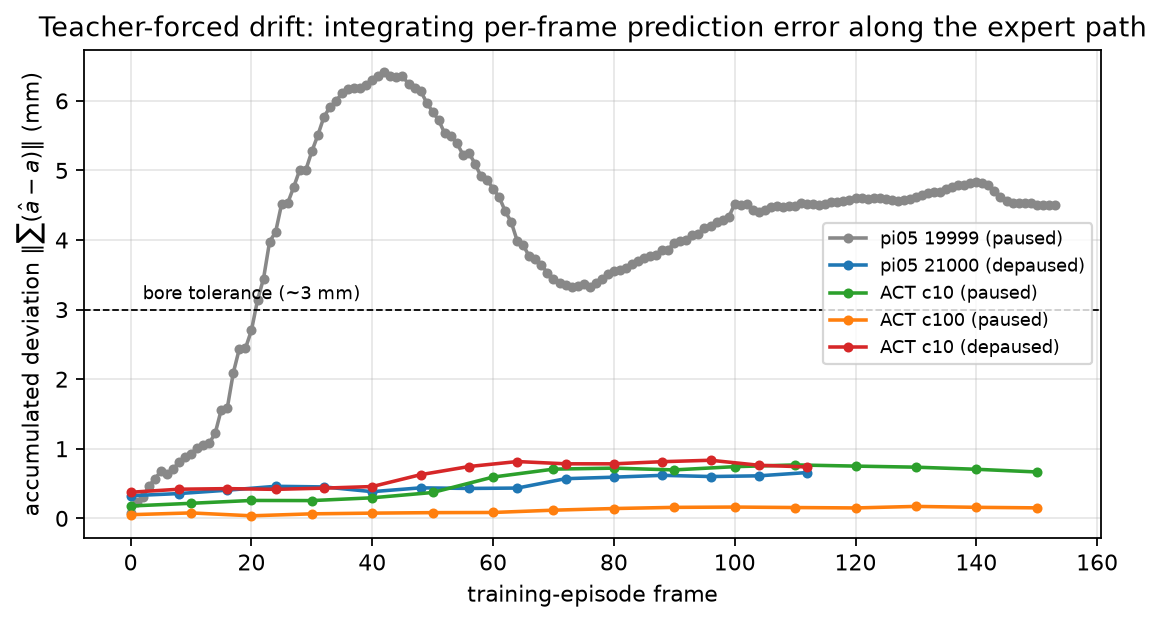
\includegraphics[width=0.78\textwidth]{openloop_drift.png}
\caption{Teacher-forced drift: accumulated prediction error
$\lVert\sum_t(\hat a_t - a_t)\rVert$ along the expert path. On-path predictions are
nearly unbiased for all but the paused $\pi_{0.5}$; the closed-loop lateral
blow-ups are feedback amplification of small errors in off-path states the
datasets never cover, not an open-loop bias.}
\label{fig:drift}
\end{figure}

\subsection{Closed-loop rollouts}
Table~\ref{tab:closed} and Fig.~\ref{fig:traces} summarize one rollout per model on
identical training-episode conditions ($N{=}1$; a 40-episode matrix over train and
held-out conditions is in progress).

\begin{table}[h]\centering\small
\begin{tabular}{lllll}
\toprule
model & data & behavior & best position & seated \\
\midrule
$\pi_{0.5}$ 5k--20k  & original & stalls at $-19$\,mm, bounces & never enters & no \\
$\pi_{0.5}$ 21000    & depaused & drives, drifts past jack     & 4.7\,mm @ 10\,mm lat & no \\
ACT c10              & original & \textbf{slow, holds alignment} & \textbf{9.7\,mm @ 5.8\,mm lat}$^{*}$ & no \\
ACT c100             & original & blind 100-step chunks drift  & 7.8\,mm @ 10\,mm lat & no \\
ACT c10              & depaused & perfect pre-dock, then drifts & $-17.9$\,mm @ 3.0\,mm lat$^{\dagger}$ & no \\
\bottomrule
\end{tabular}
\caption{Closed-loop rollouts, training-episode conditions, 450-step budget.
$^{*}$still advancing at budget expiry. $^{\dagger}$best-aligned pre-dock of any
run (step 40), lost during the push.}
\label{tab:closed}
\end{table}

\begin{figure}[h]\centering
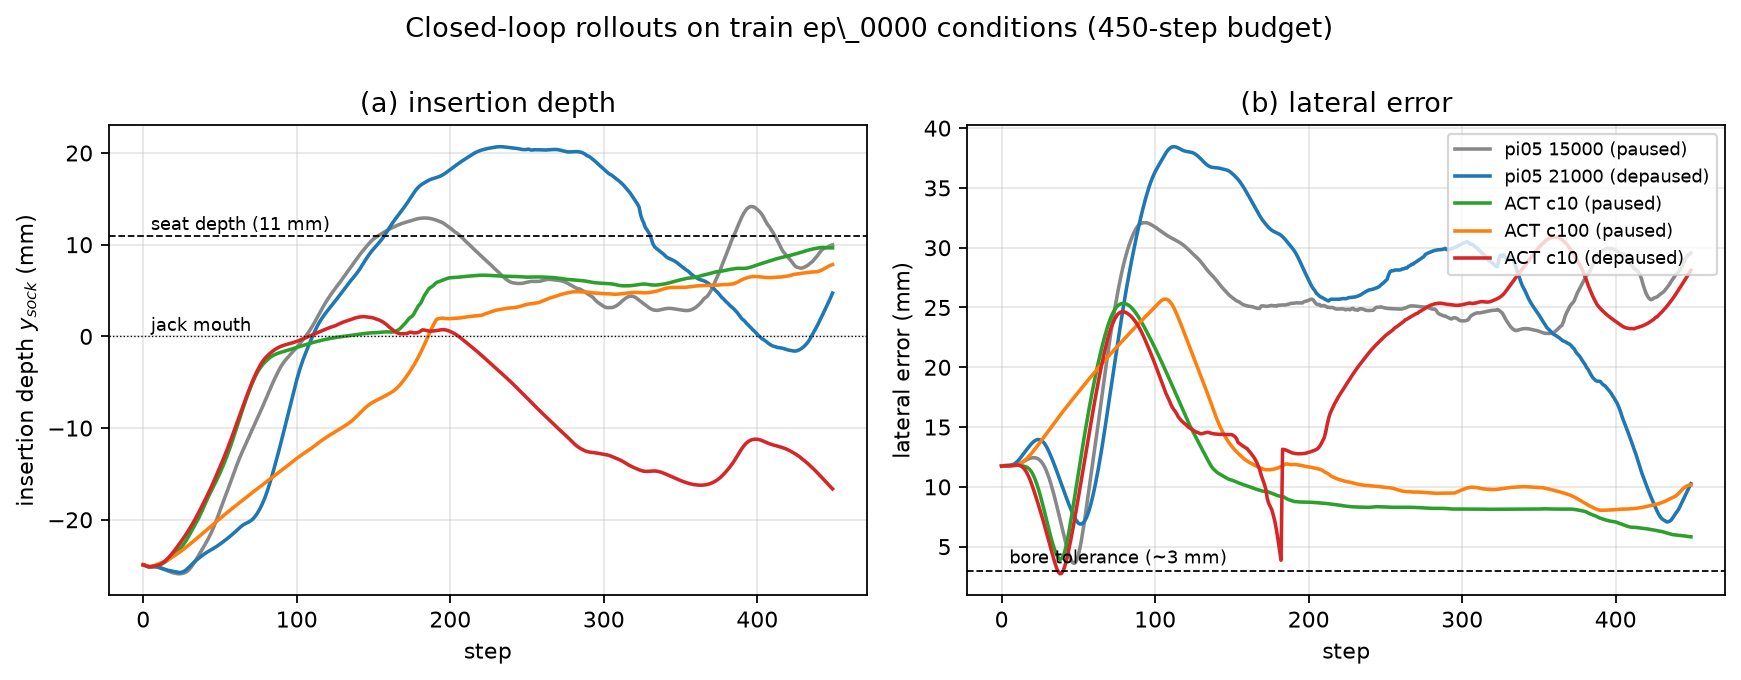
\includegraphics[width=\textwidth]{closed_loop_traces.png}
\caption{Closed-loop traces. (a) The paused $\pi_{0.5}$ never passes the pre-dock;
depaused models advance but (b) their lateral error diverges far beyond the bore
tolerance. The paused ACT c10 is the only run that keeps lateral error near
tolerance while advancing.}
\label{fig:traces}
\end{figure}

\subsection{Findings}
\begin{enumerate}\itemsep2pt
  \item \textbf{The pause pathology is real but architecture-dependent.} Motionless
        pre-dock frames taught $\pi_{0.5}$ an absorbing ``output zero'' state
        (closed-loop stall); ACT, trained on the same data, averages through it.
  \item \textbf{De-pausing trades stall for imprecision.} With the 0.2\,mm floor both
        architectures move decisively but lose slow fine alignment: both depaused
        models blow through or around the jack. This motivated the gentler
        \texttt{dp01} variant.
  \item \textbf{The universal failure is uncorrected lateral drift.} Every model,
        both architectures, both datasets: once off the demonstrated path, none
        returns to it. Combined with Fig.~\ref{fig:drift}, the failure lives
        entirely in off-path states, not per-step accuracy --- the datasets contain
        zero return-to-path demonstrations (classic BC compounding). An in-progress
        recovery campaign ($\sim$562 episodes: near-dock off-nominal starts and
        mid-flight perturbation kicks, episodes split at the kick so only the
        correction is labeled) targets exactly these states.
\end{enumerate}
% ---------------------------------------------------------------------------
